\chapter{\label{ch3-architecture}CTA Architecture} 

\minitoc

\notes[inline,caption={}]{
	\section{Plan}
	\subsection{Topics}
	\begin{itemize}
		\item Requirements
		\item Data Levels
	\end{itemize}
	\subsection{Questions}
	\begin{itemize}
		\item ?
	\end{itemize}
}

\section{Introduction}

Due to the large scope of \gls{cta}, in both its construction and operation, a formal approach towards a system architecture was adopted \cite{Dazzi2018}. One important aspect within this architecture is the distinction between the \gls{cta} Consortium and the \gls{cta} Observatory. The \gls{cta} Consortium is a group of institutes responsible for directing the science goals of the observatory, and for developing software and hardware (including cameras), which are supplied to the observatory as in-kind contributions. The consortium consists of 200 institutes across 31 countries \cite{cta-consortium}. Conversely, the CTA Observatory pertains to the major astronomical facility that serves science data to a wide user community as an open observatory. The \gls{cta} Observatory gGmbH is the legal entity for \gls{cta} in the preparation for the implementation of the \gls{cta} Observatory, and works in close cooperation with the consortium during this process \cite{cta-observatory}.

The purpose of the \gls{cta} architecture is to maintain communication and understanding among all \gls{cta} contributors during the pre-construction phase in order to ensure a coherent development process and seamless integration of the developed units into a whole. During this chapter I will describe two aspects of the \gls{cta} architecture that are important in the context of this thesis: certain requirements that all cameras, including \gls{chec}, must meet; and the descriptions of how camera-observation data are handled in \gls{cta}, including the system flow and data level definitions.

\section{Requirements}

In order to ensure the science goals of \gls{cta} are achievable, and that the observatory remains operational for the full 30 life-time, certain standards must be upheld by all components of the observatory; this is the purpose of the \gls{cta} requirements. The requirements cover every aspect of the observatory, including: the survival of environmental conditions (\textit{B-ENV-0320 Survival humidity}), the time allowed by the analysis pipeline for processing (\textit{A-OBS-0810 Data Processing Efficiency}), the reliability of telescope components (\textit{B-TEL-0520 Structure Lifetime}), and the ability to meet the expected performance (\textit{PROG-0025 Differential Sensitivity under Low Moonlight - North}). In order for an in-kind contribution to be accepted, it must meet the requirements defined by the observatory. These requirements are therefore the standards for which we compare the performance of \gls{chec} against, and are the primary drivers in my development of the low-level calibration and analysis. However, there exists more than 60 requirements specifically tailored for the cameras. Consequently, the full review of the camera is a large undertaking that extends beyond the scope of this thesis. Instead, only the requirements that have relevance to this thesis' topic are discussed.

It is important to note that the requirements, located on the \gls{cta} Jama website \cite{cta-jama}, are currently under-review and therefore subject to change. One such change that is under-way at the time of this writing is the redefinition from units of photoelectrons to photons. Originally, a common consolidated \gls{pmt} was envisioned to be used for all cameras in \gls{cta}, motivating for the expression of requirements to be in photoelectrons. However, due to the advances in sensor technology and the adoption of \glspl{sipmt}, this assumption has lead to problems with such a definition \cite{petophotons}. Firstly, a fixed \gls{nsb} level defined in terms of photoelectrons does not allow for trade-offs between \gls{nsb} acceptance and other performance parameters. Secondly, with an \gls{sipmt}-based camera it is possible to obtain a better Cherenkov intensity resolution and a lower energy threshold, but still fail the current requirements, whilst a camera design with inferior performance may pass. The current requirements could be met by a camera with subpar \glspl{sipmt} by reducing its bias voltage, which in turn reduces the optical cross-talk and photon detection efficiency, hence bringing the excess noise factor and threshold in photoelectron units down\change{talk with Tom about this, and how trigger efficiency was affected by being defined in p.e.}. While such a camera meets the current requirements, it is at the cost of performance in terms of photon intensity (and therefore Cherenkov-shower energy threshold). 

A copy of each requirement at the time of this writing is included alongside the discussion in this section to ensure clarity about which version of the requirement definition is being referred to. Future investigations should check the latest requirement definition. \vfill

\begin{requirement}{\subsection{B-TEL-1010 Charge Resolution}}
	The required fractional Charge Resolution for Cherenkov signals in each Camera pixel for a specified background level of 0.125 photoelectrons/ns is given in the Figure below and Table attached. Charge measurements must be possible for 0-1000 photoelectron signals. The average charge resolution should be calculated for the reference Gamma-Ray Spectrum.
    
	\centering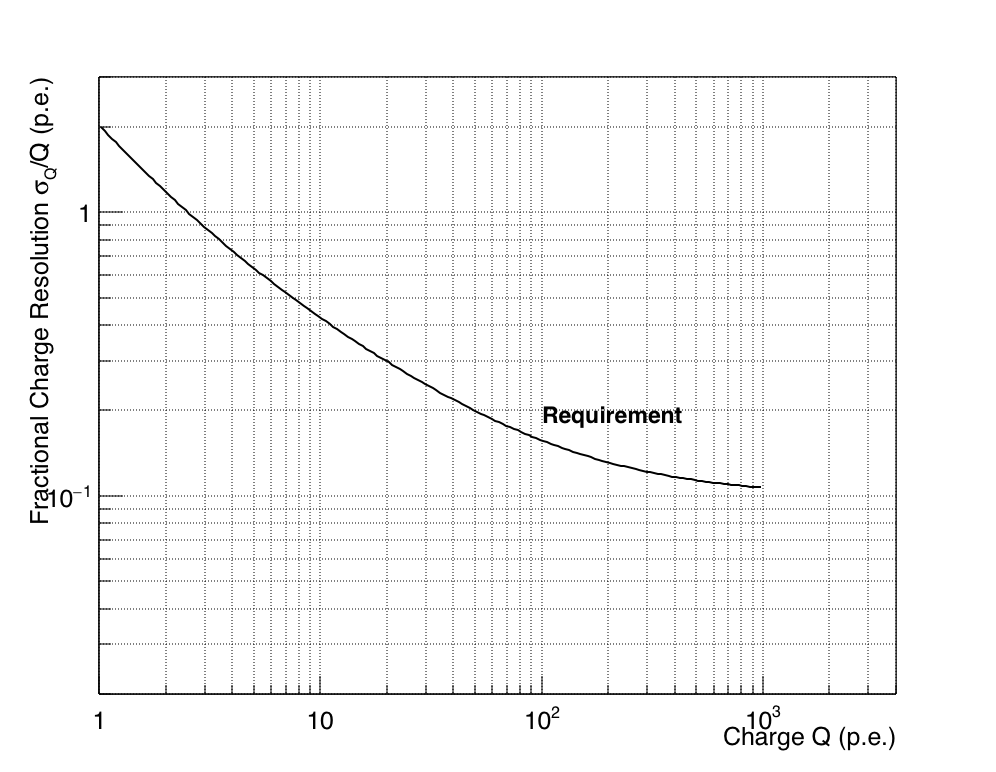
\includegraphics[width=0.8\linewidth]{figures/images/charge_res_req}
	\captionof{figure}{Fractional rms charge resolution $\sigma_Q/Q$ per pixel for different Cherenkov light signal amplitudes, expressed in units of photoelectrons (p.e.). All sources of fluctuations, including Poisson fluctuations in photoelectron number, must be included, The true pixel charge $Q$ is that measured in an ideal detector with the same photon-detection efficiency. }\label{fig:charge_res_req}
    
\begin{itemize}
\item [Notes:] It is expected that this requirement is verified with reference to:

- Monte Carlo simulation of Cherenkov light from gamma-ray initiated showers (using a verified telescope model),

- Level-C Specification on Laboratory Measured Charge Resolution,

- Monte Carlo simulation of the laboratory test set-up (as a means of telescope model verification).

Note that between 1000~p.e. and 2000~p.e., some sensitivity to increasing input signal must exist. \newline
This requirement applies to post-calibration (DL1) data. \newline
Note that this requirement will likely need to be expanded to cover performance at higher NSB levels.
\end{itemize}
\end{requirement}

\subsubsection{Definition}
The standard criterion for low-level performance used in \gls{cta} is the \textit{Charge Resolution}. It encompasses both the bias and the standard deviation of the extracted charge versus the expected charge to provide a measure of the waveform, calibration, and charge reconstruction quality. Analogous to the Root-Mean-Square Error, the fractional \textit{Charge Resolution} $\dfrac{\sigma_Q}{Q_T}$ for a particular ``true charge'' $Q_T$ (the charge that would be measured directly after the photocathode of the sensor) is defined as
\begin{equation} \label{eq:charge_res}
\dfrac{\sigma_Q}{Q_T} = \dfrac{1}{Q_T} \sqrt{\dfrac{\sum_{i=0}^N (Q_{M_i} - Q_T)^2}{N}},
\end{equation}
where $N$ is the total number of measured charges, $Q_{M_i}$, with that value of $Q_T$. The associated \gls{cta} requirement defines the maximum allowed values of $\dfrac{\sigma_Q}{Q_T}$ for values of $Q_T$ between 1-1000~p.e., which must be adhered to when resolving the signal for any camera in \gls{cta}.

\subsubsection{Requirement Derivation}
The uncertainty in charge reconstruction can be expressed in the form
\begin{equation} \label{eq:charge_res_req}
\dfrac{\sigma_Q}{Q} = \dfrac{1}{Q} \sqrt{\sigma_0^2 + \sigma_{ENF}^2 Q + \sigma_g^2 Q^2},
\end{equation}
where $\sigma_0$ encapsulates noise contributions (electronic and \gls{nsb}), $\sigma_{ENF} = 1 + \mathit{ENF}$ is determined from the \textit{Excess Noise Factor} (a measure of the avalanche gain fluctuations), and $\sigma_g$ is the multiplicative errors of the gain \cite{petophotons}\cite{Ohm2012}. $\sigma_0$ can be further expanded in terms of the two primary noise contributions:
\begin{equation} \label{eq:charge_res_nsb}
\sigma_0 = \sqrt{\mathit{NSB} \times t_w + n_e^2},
\end{equation}
i.e. the $\mathit{NSB}$ rate (which includes the \gls{dcr} for the purpose of this discussion) is coupled with the effective signal readout window size, $t_w = 15$ ns, and summed with the electronic noise, $n_e$. A contribution from electronic noise of $n_e = 0.87$ photoelectrons is assumed, combined with a value of $\mathit{NSB} = 0.125$ p.e./ns as defined in the requirement. A value of $\sigma_g = 0.1$ and $\mathit{ENF} = 0.2$ is also assumed \cite{petophotons}. The resulting combination of miscalibration and noise factors in Equation~\ref{eq:charge_res_req} gives the \textit{Charge Resolution} requirement illustrated in Figure~\ref{fig:charge_res_req}.

\subsubsection{Approach}
As it is impossible to know the ``true charge'' generated by a Cherenkov signal in the field, Monte Carlo simulations must be relied upon in order to prove a camera meets this requirement. The process for achieving this is outlined in the notes to the requirement. It is expected that this requirement is validated in three ways:
\begin{enumerate}
\item With lab measurements where the camera in uniformly illuminated with a calibrated light-source.
\item With simulations of the previous approach, in order to verify the simulation model of the camera.
\item With Monte Carlo simulations of Cherenkov signal incident on the full telescope model.
\end{enumerate}
The final item is the most important in confirming the requirements are met, as temporally-uniform illuminations do not sufficiently test the ability to find the signal pulse in the waveforms for the case of a Cherenkov-shower illumination. 

The software package \textit{sim\_telarray} (Chapter~\ref{ch4-software}) stores the ``true charge'' generated after the photocathode for each shower event into the output file. Therefore, with an accurately simulation model of the camera, it is an appropriate package for investigating a camera's performance against this requirement. However, in order to ensure Poisson fluctuations in photoelectron number are included, as per the requirement, when using the ``true charge'' stored in the simulation file, the corrected form of Equation~\ref{eq:charge_res} is
\begin{equation} \label{eq:charge_res2}
\dfrac{\sigma_Q}{Q_T} = \dfrac{1}{Q_T} \sqrt{\dfrac{\sum_{i=0}^N (Q_{M_i} - Q_T)^2}{N} + Q_T}.
\end{equation}
With the form in Equation~\ref{eq:charge_res2}, a perfect detector that consistently reads-out a ``measured charge'' with equal value to the ``true charge'' would hit the Poisson limit, as it is not physically possible to know the the ``true charge'' generated by the photocathode without fluctuations. The Poisson limit is shown alongside the \textit{Charge Resolution} requirement in Figure~\change{figure showing the two limit lines}.

\section{Data Levels}

